\chapter{Append}
\label{AppChap:Robustness}

\section{Robustness}

\begin{figure}[ht]
    \centering
    \begin{subfigure}{0.48\textwidth}
        \centering
        \includegraphics[width = \textwidth]{C:/Users/leonh/Desktop/Praktikum_AWI/NordPolLinks/Lon_66_70/TMin/TMin_Month_9.png}
        \caption{$T_{min}$ for the left hemisphere between 66 and 70°}
    \end{subfigure}
    \begin{subfigure}{0.48\textwidth}
        \centering
        \includegraphics[width = \textwidth]{C:/Users/leonh/Desktop/Praktikum_AWI/NordPolRechts/Lon_66_70/TMin/TMin_Month_9.png}
        \caption{$T_{min}$ for the right hemisphere between 66 and 70°}
    \end{subfigure}
    
    \begin{subfigure}{0.48\textwidth}
        \centering
        \includegraphics[width = \textwidth]{C:/Users/leonh/Desktop/Praktikum_AWI/NordPolLinks/Lon_70_75/TMin/TMin_Month_9.png}
        \caption{$T_{min}$ between 70 and 75°}
    \end{subfigure}
    \begin{subfigure}{0.48\textwidth}
        \centering
        \includegraphics[width = \textwidth]{C:/Users/leonh/Desktop/Praktikum_AWI/NordPolRechts/Lon_70_75/TMin/TMin_Month_9.png}
        \caption{$T_{min}$ between 70 and 75°}
    \end{subfigure}

        
    \begin{subfigure}{0.48\textwidth}
        \centering
        \includegraphics[width = \textwidth]{C:/Users/leonh/Desktop/Praktikum_AWI/NordPolLinks/Lon_75_80/TMin/TMin_Month_9.png}
        \caption{$T_{min}$ between 75 and 80°}
    \end{subfigure}
    \begin{subfigure}{0.48\textwidth}
        \centering
        \includegraphics[width = \textwidth]{C:/Users/leonh/Desktop/Praktikum_AWI/NordPolRechts/Lon_75_80/TMin/TMin_Month_9.png}
        \caption{$T_{min}$ between 75 and 80°}
    \end{subfigure}

    \begin{subfigure}{0.48\textwidth}
        \centering
        \includegraphics[width = \textwidth]{C:/Users/leonh/Desktop/Praktikum_AWI/NordPolLinks/Lon_80_82/TMin/TMin_Month_9.png}
        \caption{$T_{min}$ between 80 and 82°}
    \end{subfigure}
    \begin{subfigure}{0.48\textwidth}
        \centering
        \includegraphics[width = \textwidth]{C:/Users/leonh/Desktop/Praktikum_AWI/NordPolRechts/Lon_80_82/TMin/TMin_Month_9.png}
        \caption{$T_{min}$ between 80 and 82°}
    \end{subfigure}
    % Include your other subfigures here...
    \caption{Temperature for left and right hemisphere}
    \label{app:MinTemp}
\end{figure}

\begin{figure}[ht]
    \centering
    \begin{subfigure}{0.48\textwidth}
        \centering
        \includegraphics[width = \textwidth]{C:/Users/leonh/Desktop/Praktikum_AWI/NordPolLinks/Lon_66_70/TMax/TMax_Month_9.png}
        \caption{$T_{max}$ for the left hemisphere between 66 and 70°}
    \end{subfigure}
    \begin{subfigure}{0.48\textwidth}
        \centering
        \includegraphics[width = \textwidth]{C:/Users/leonh/Desktop/Praktikum_AWI/NordPolRechts/Lon_66_70/TMax/TMax_Month_9.png}
        \caption{$T_{max}$ for the right hemisphere between 66 and 70°}
    \end{subfigure}
    
    \begin{subfigure}{0.48\textwidth}
        \centering
        \includegraphics[width = \textwidth]{C:/Users/leonh/Desktop/Praktikum_AWI/NordPolLinks/Lon_70_75/TMax/TMax_Month_9.png}
        \caption{$T_{max}$ between 70 and 75°}
    \end{subfigure}
    \begin{subfigure}{0.48\textwidth}
        \centering
        \includegraphics[width = \textwidth]{C:/Users/leonh/Desktop/Praktikum_AWI/NordPolRechts/Lon_70_75/TMax/TMax_Month_9.png}
        \caption{$T_{max}$ between 70 and 75°}
    \end{subfigure}

        
    \begin{subfigure}{0.48\textwidth}
        \centering
        \includegraphics[width = \textwidth]{C:/Users/leonh/Desktop/Praktikum_AWI/NordPolLinks/Lon_75_80/TMax/TMax_Month_9.png}
        \caption{$T_{max}$ between 75 and 80°}
    \end{subfigure}
    \begin{subfigure}{0.48\textwidth}
        \centering
        \includegraphics[width = \textwidth]{C:/Users/leonh/Desktop/Praktikum_AWI/NordPolRechts/Lon_75_80/TMax/TMax_Month_9.png}
        \caption{$T_{max}$ between 75 and 80°}
    \end{subfigure}

    \begin{subfigure}{0.48\textwidth}
        \centering
        \includegraphics[width = \textwidth]{C:/Users/leonh/Desktop/Praktikum_AWI/NordPolLinks/Lon_80_82/TMax/TMax_Month_9.png}
        \caption{$T_{max}$ between 80 and 82°}
    \end{subfigure}
    \begin{subfigure}{0.48\textwidth}
        \centering
        \includegraphics[width = \textwidth]{C:/Users/leonh/Desktop/Praktikum_AWI/NordPolRechts/Lon_80_82/TMax/TMax_Month_9.png}
        \caption{$T_{max}$ between 80 and 82°}
    \end{subfigure}
    % Include your other subfigures here...
    \caption{Temperature for left and right hemisphere}
    \label{app:MaxTemp}
\end{figure}


\clearpage
\section{Local observations}

\begin{figure}[h!]
    \centering
    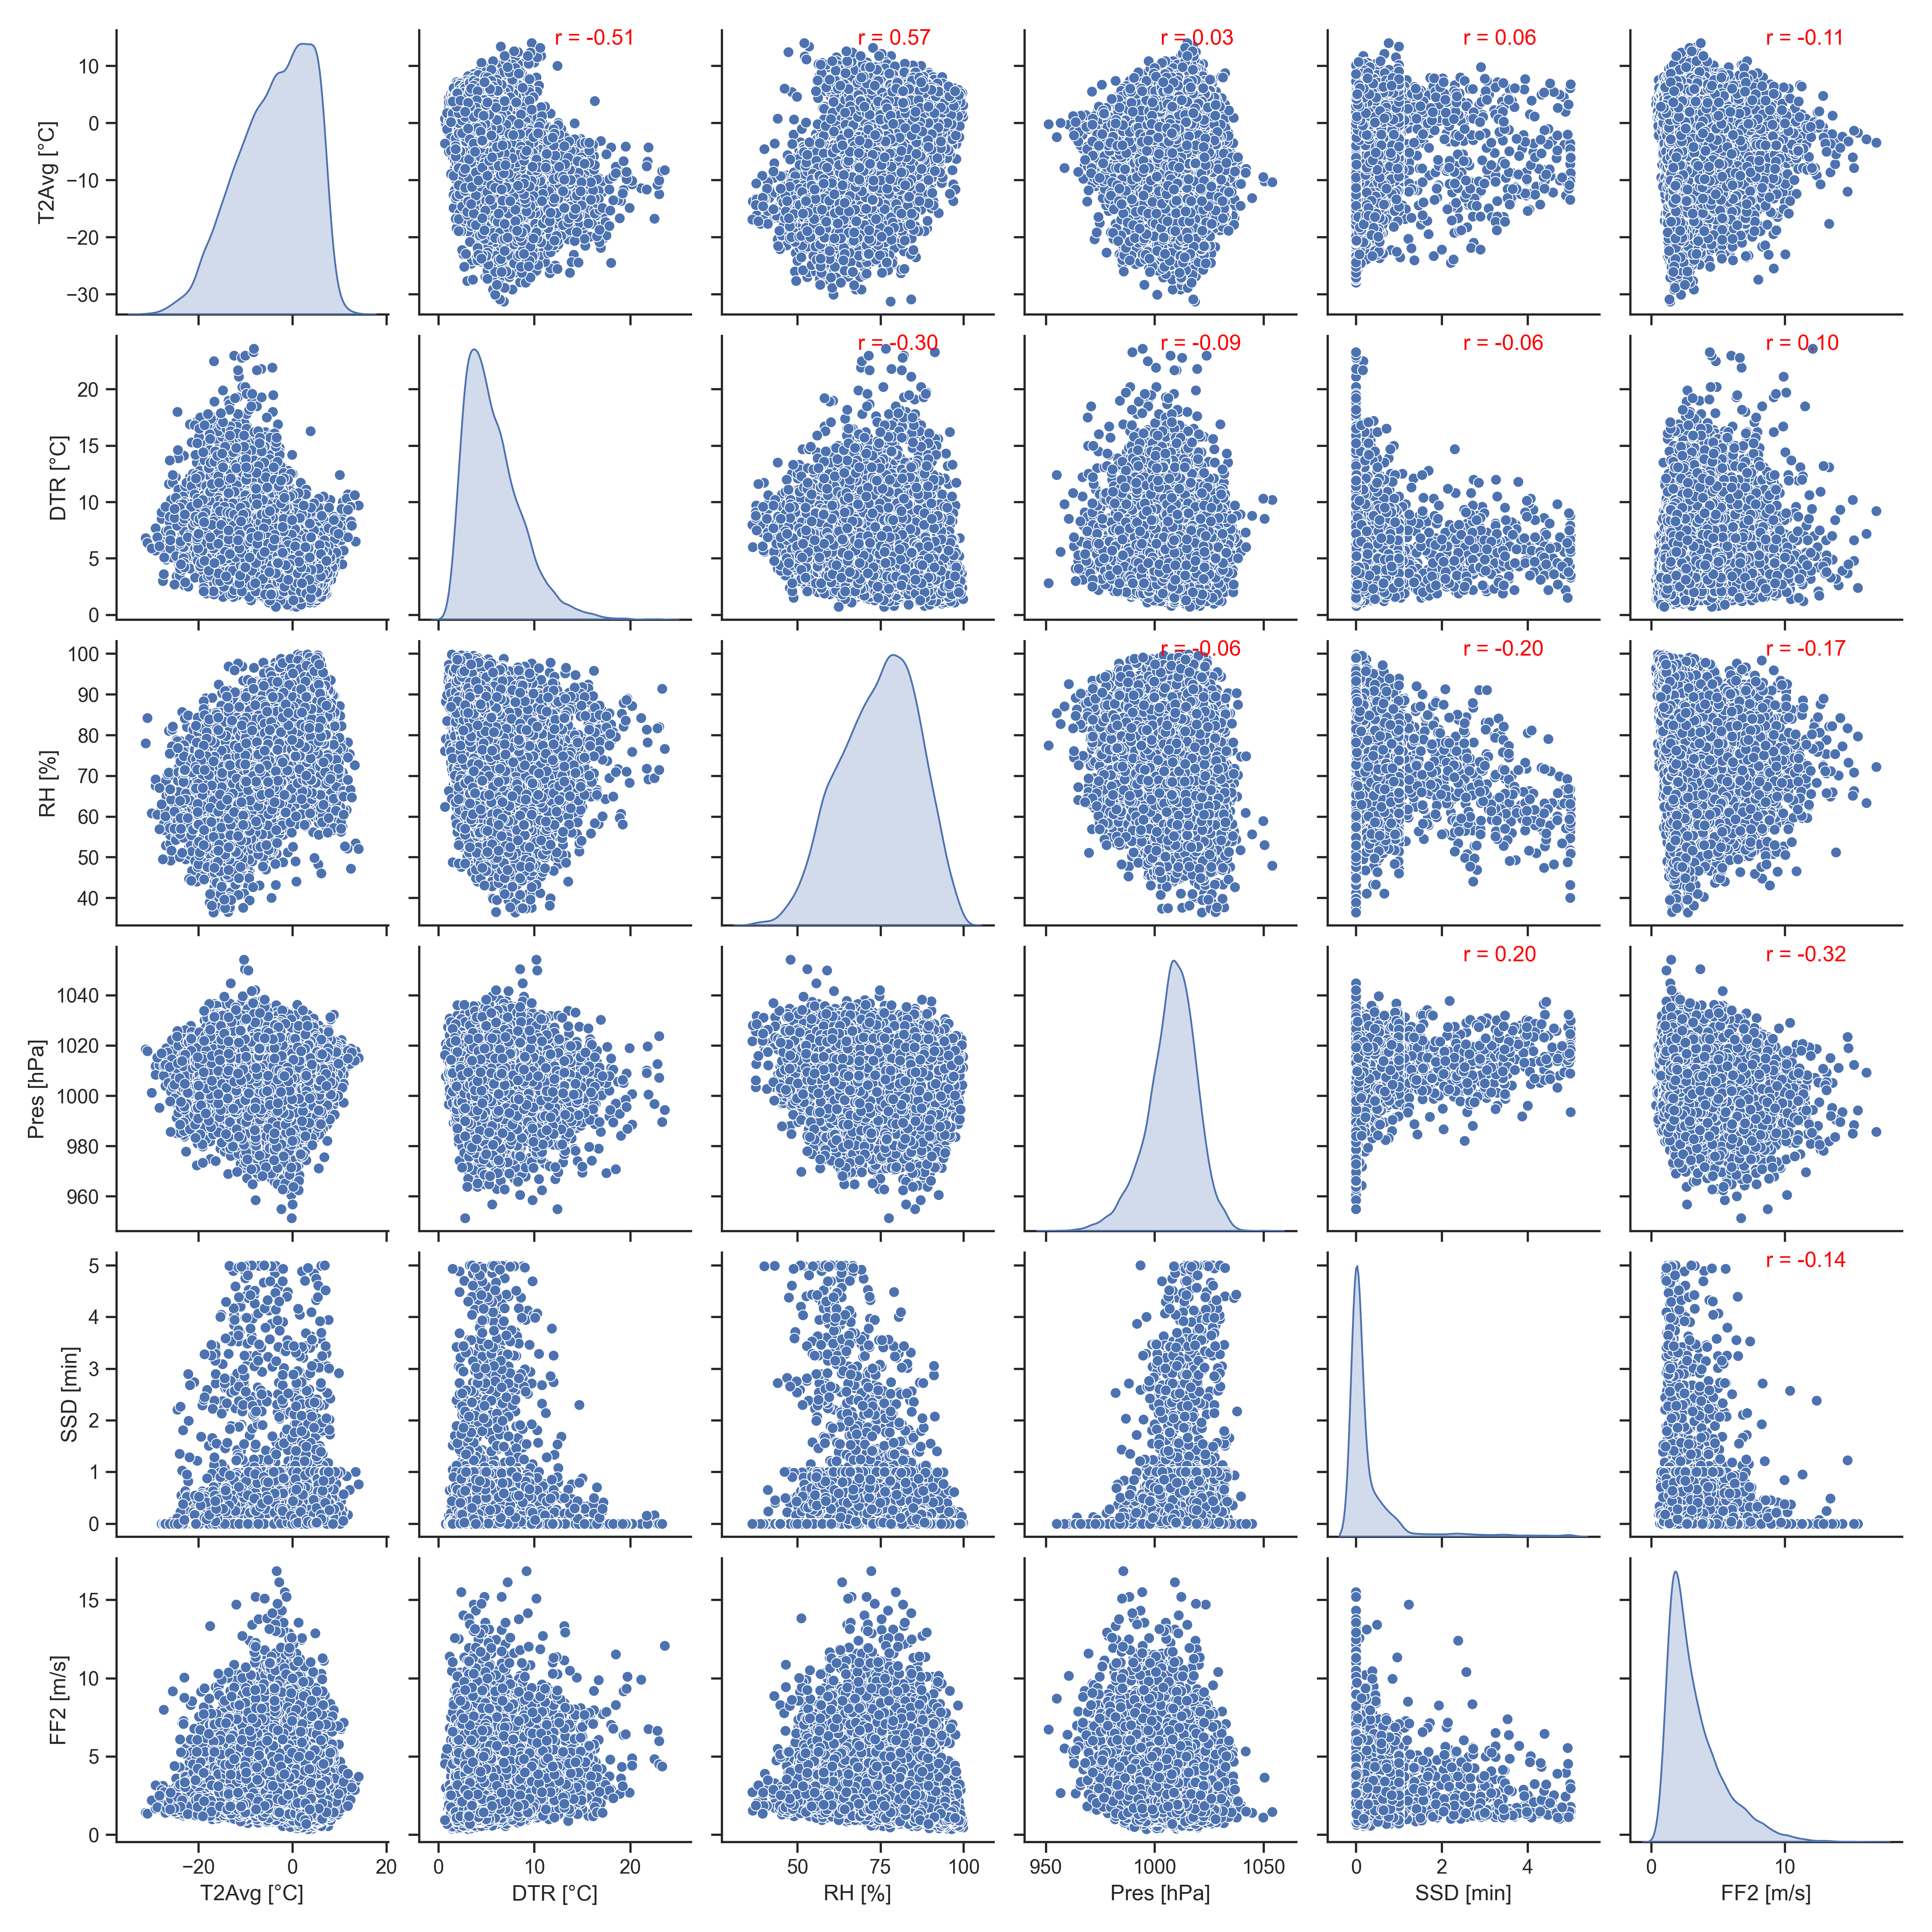
\includegraphics[width = \textwidth]{C:/Users/leonh/Desktop/Praktikum_AWI/Spitzbergen/SB_correlations_days.png}
    \caption{Comparing daily Diurnal Temperature Ranges with Average Daily Temperatures at Arctic Meteorological Station from AWIPEV from 1983 to 2022}
    \label{fig:SB_DTR_days_scatterd}
\end{figure}\


\begin{figure}[h!]
    \centering
    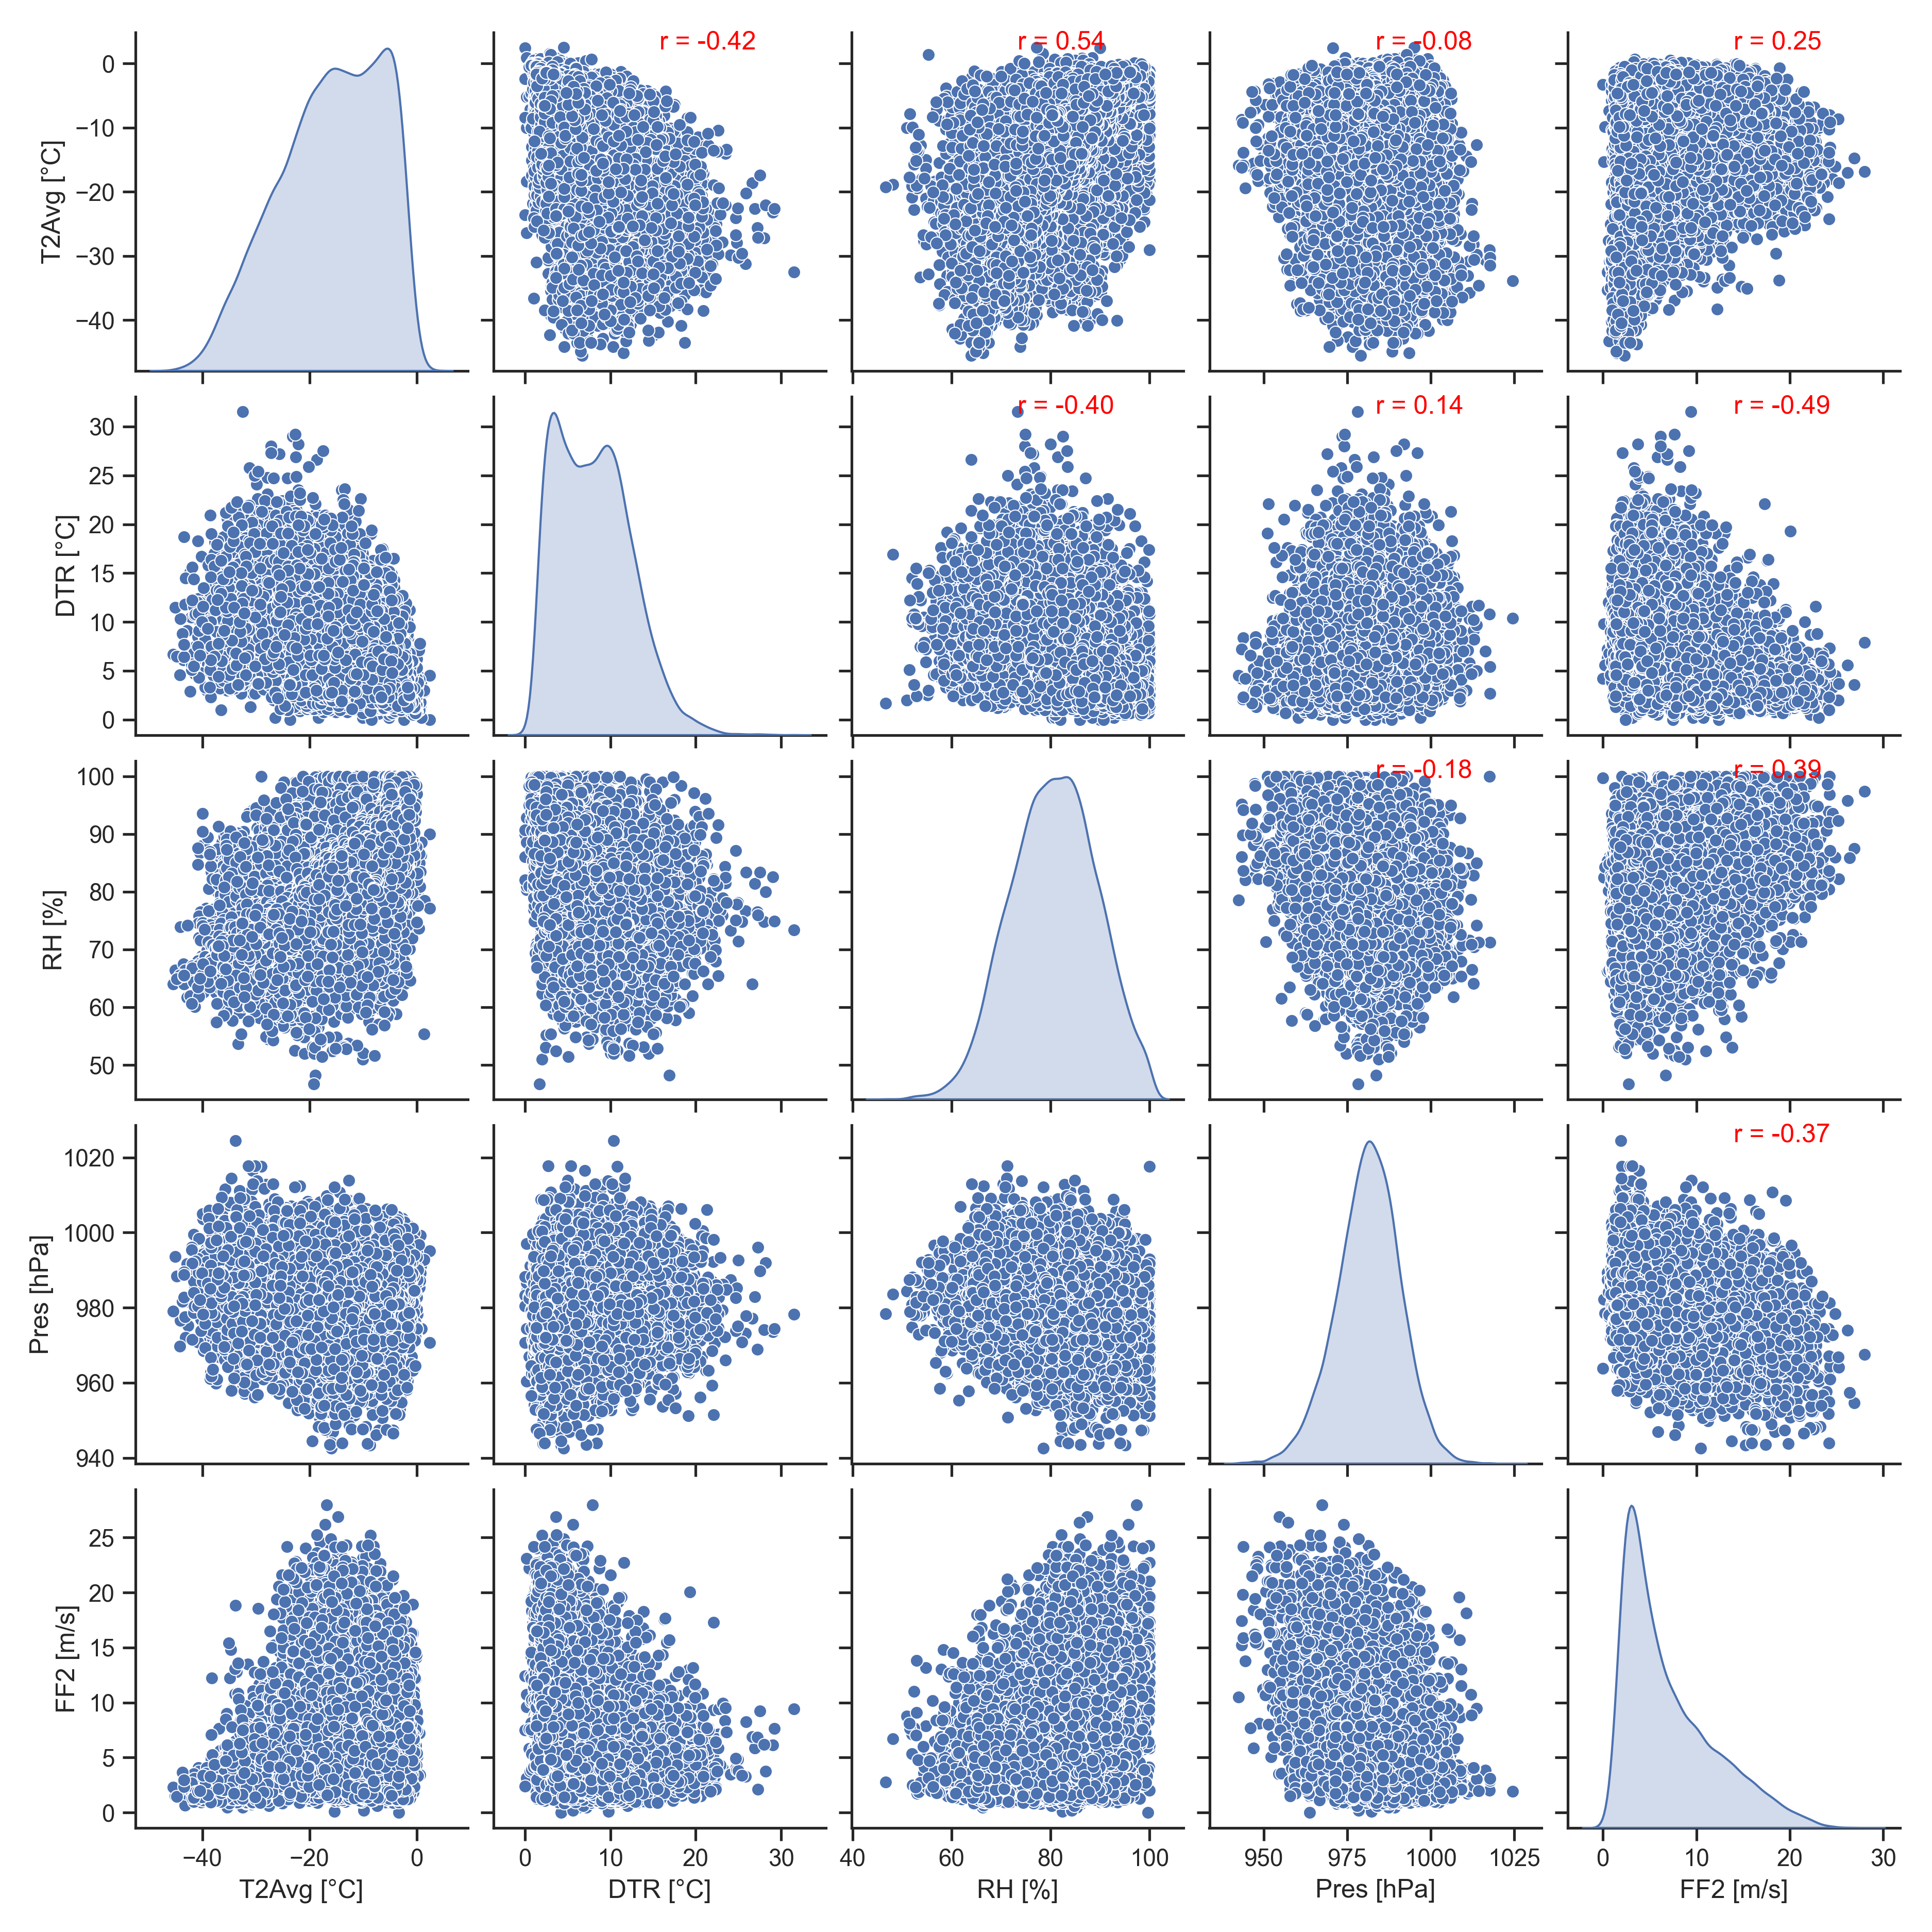
\includegraphics[width = \textwidth]{C:/Users/leonh/Desktop/Praktikum_AWI/GVN/GVN_correlation_days.png}
    \caption{Comparing daily Diurnal Temperature Ranges with Average Daily Temperatures at Antarctica's Neumayer Meteorological Station from 1983 to 2022}
    \label{fig:GVN_DTR_days_scatterd}
\end{figure}\

